% Difference between living documentation and testing
% Difference between BDD and TDD

\chapter*{Is BDD the same as Test Automation?}

\ifnotes
    Learning outcomes:
    
    \begin{itemize}
        \item Reiterate that Automation is the last of the three practices of BDD
        \item Explain that feature files are documentation/specifications NOT test scripts
        \item Describe why scenarios are equivalent to acceptance tests
        \item Agree that not all testing can be automated
        \item Describe the benefits of living documentation
        \item List three forms of automation that is not driven by feature files (load, penetration, programmer)
        \item Explain that the key difference between TDD and BDD is the people who will be able to contribute feedback
        \item Explain the Red/Green/Refactor loop
        \item Confirm that dev and test need to collaborate closely to build trust
    \end{itemize}
    
    
    Setup:
    
        Run this as an Interactive Lecture using the Beat The Clock approach from LFTBOTR. Ask lots of questions, such as:
        
        \begin{itemize}
            \item what would you describe a features file as? spec, doc, tests?
            \item if you automate your feature files will you need other forms of testing?
            \item can anyone explain TDD
            \item explain why green should be "shameless" and should take a v. short time
            \item define "refactor"
            \item why should you only refactor from green?
            \item can you think of another way to describe "write a test" [A: write next (micro) specification]
            \item why do we need automated tests for clean code? what is clean code? why can't we be agile without clean code?
        \end{itemize}
        
        They get 60 seconds at the end to write down 10 important facts that they have heard.
\fi 

\ifcontent

    \emph{Automation} is mainly of interest to developers and automation engineers, but there are some concepts that the whole team should be comfortable with.
    
    \QandAbox{First lets consider the relationship between \emph{living documentation} and \emph{software testing}. Make notes in the box}{5}
    
    Now, let's discuss the relationship between \emph{BDD} and \emph{TDD}. \\

    \begin{center}
        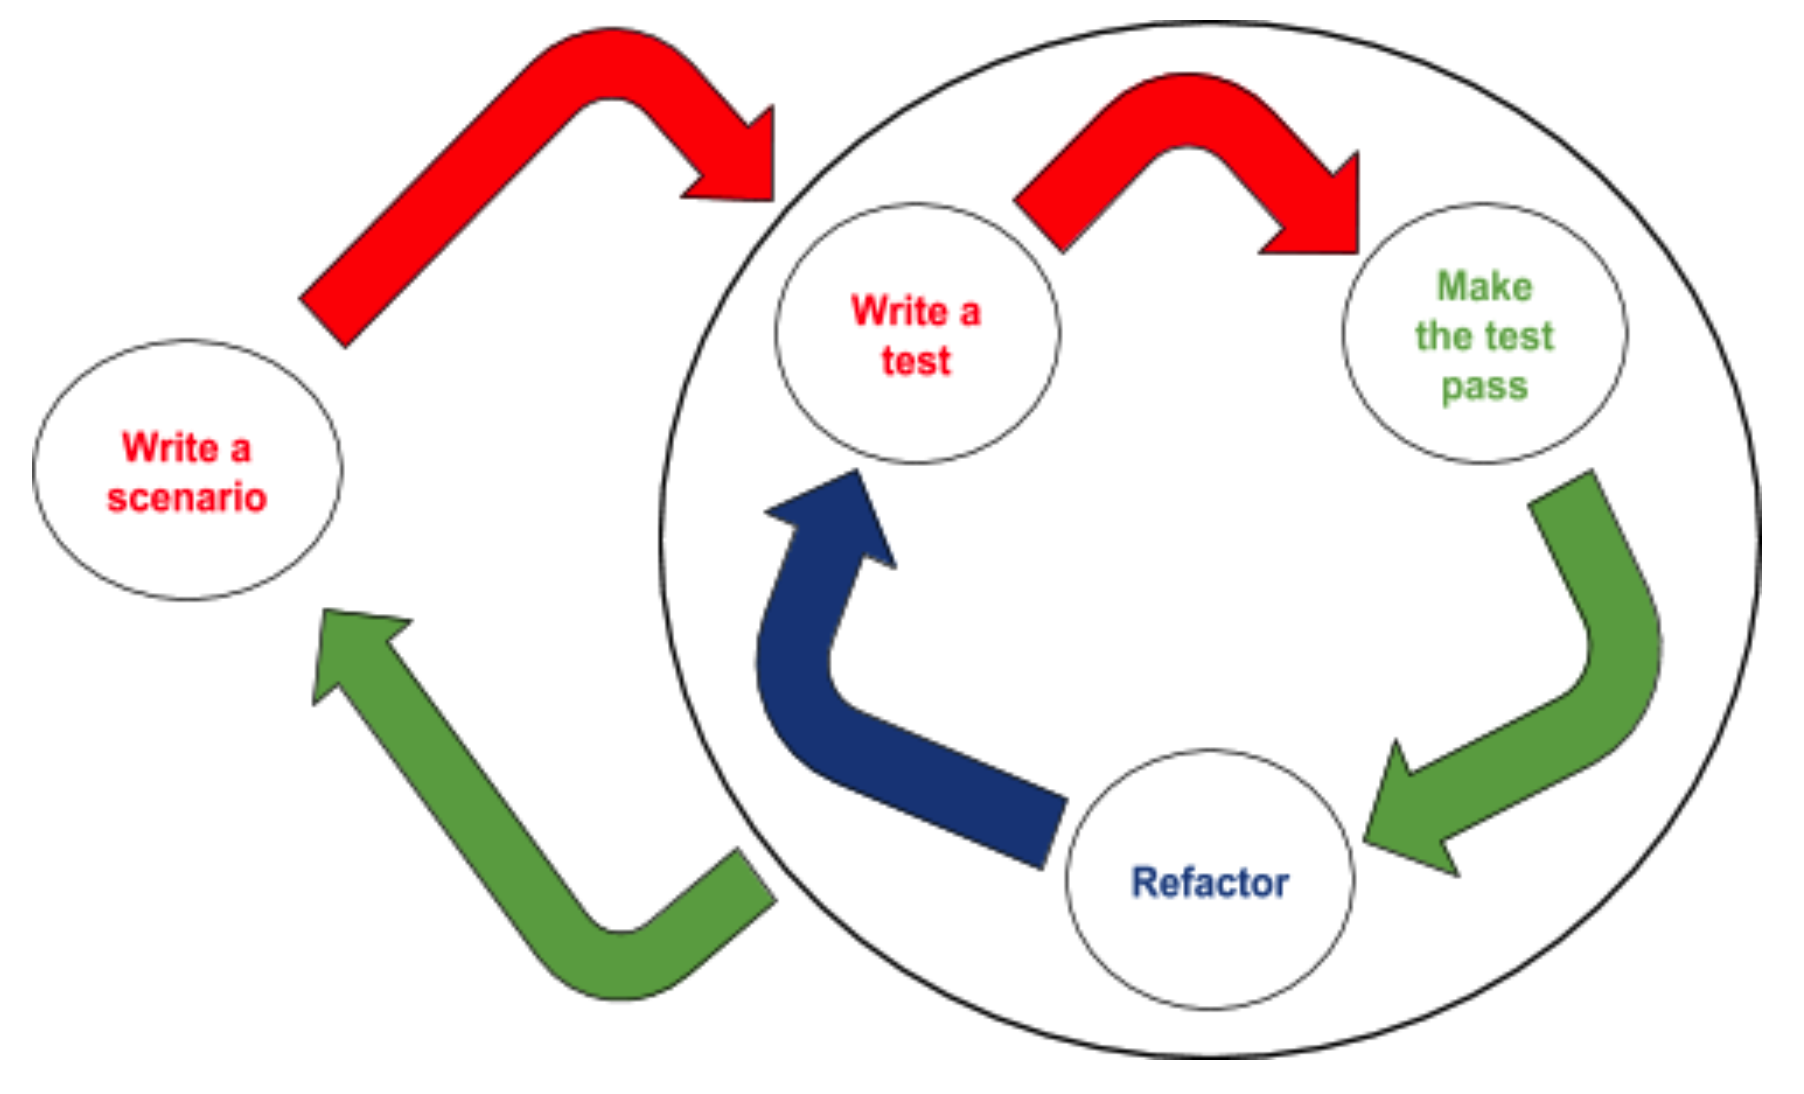
\includegraphics[width=0.6\textwidth]{bdd-fundamentals/images/BDD-TDD-loop.png}
    \end{center}

    \QandAbox{Make notes on the diagram above, or in the box below}{5}
    

    \chapter*{Beat the clock}
    
        List the ten most important facts that you've just learnt: \\
        \begin{framed}
            1 \\
              \\
              \\
              \\
            2 \\
              \\
              \\
              \\
            3 \\
              \\
              \\
              \\
            4 \\
              \\
              \\
              \\
            5 \\
              \\
              \\
              \\
            6 \\
              \\
              \\
              \\
            7 \\
              \\
              \\
              \\
            8 \\
              \\
              \\
              \\
            9 \\
              \\
              \\
              \\
            10\\
              \\
              \\
              \\
        \end{framed}    
\fi